\documentclass[letterpaper,twocolumn,amsmath,amssymb,prb]{revtex4-1}
\usepackage{graphicx}% Include figure files
\usepackage{dcolumn}% Align table columns on decimal point
\usepackage{bm}% bold math
\usepackage{color}

%%%%%%%%%%%%%%%%%%%%%%%%%%%%%%%%%%%%%%%%%%%%%%%%%%%%%%%%%%%%
%% Definitions
\def\re{\text{Re}}
\def\im{\text{Im}}
\def\ket#1{\vert #1 \rangle}
\def\cU{{\cal{U}}}
\def\cD{{\cal{D}}}
\def\re{\text{Re}}
\def\im{\text{Im}}
\newcommand{\red}[1]{{\bf \color{red} #1}}
\newcommand{\blue}[1]{{\bf \color{blue} #1}}
\newcommand{\green}[1]{{\bf \color{green} #1}}
\newcommand{\rr}{\textbf{r}}
\newcommand{\xx}{\textbf{r}}
\newcommand{\refnote}{\red{[ref]}}

% fixme is intended to prioritize stuff that needs fixing.
\newcommand{\fixme}[1]{\textcolor{red}{[\emph{#1}]}}

%%%%%%%%%%%%%%%%%%%%%%%%%%%%%%%%%%%%%%%%%%%%%%%%%%%%%%%%%%%%

\begin{document}
\title{A Classical Density-Functional Theory for Describing Water Interfaces}

\author{Jessica Hughes}
\affiliation{Department of Physics, Oregon State University, Corvallis, OR 97331}
\author{Eric Krebs}
\affiliation{Department of Physics, Oregon State University, Corvallis, OR 97331}
\author{David Roundy}
\affiliation{Department of Physics, Oregon State University, Corvallis, OR 97331}

%%%%%%%%%%%%%%%%%%%%%%%%%%%%%%%%%%%%%%%%%%%%%%%%%%%%%%%%%%%%
\begin{abstract}
We develop a classical density functional for water which combines the
White Bear fundamental-measure theory (FMT)
functional\cite{roth2002whitebear} for the hard sphere fluid with
attractive interactions based on the Statistical Associating Fluid
Theory (SAFT-VR)\cite{clark2006developing}.
This functional reproduces the properties of water at both long and
short length scales over a wide range of temperatures, and is
efficient to evaluate computationally, comparable to the cost of FMT
itself.  We demonstrate our functional by applying it to systems
composed of of two hard rods, four hard rods arranged in a square and
hard spheres in water.
\end{abstract}
\maketitle

%%%%%%%%%%%%%%%%%%%%%%%%%%%%%%%%%%%%%%%%%%%%%%%%%%%%%%%%%%%%
\section{Introduction}

A large fraction of interesting chemistry---including all of molecular
biology---takes place in aqueous solution.  However, while quantum
chemistry now enables us to calculate the ground state energies of
large molecules in vacuum, prediction of the free energy of even the
smallest molecules in the presence of a solvent poses a continuing
challenge due to the complex structure of a liquid and the
computational cost of \emph{ab initio} molecular
dynamics~\cite{car1985, grossman2004}.  The current state-of-the art
in \emph{ab initio} molecular dynamics is limited to around 64 water
molecules per unit cell, which places the minimum solute concentration
at 0.84 molar and allows contact between the second solvation shell of
neighboring solutes~\cite{izvekov2005, choe2007}\fixme{Look up more
  recent numbers on this!}.  On top of this, standard \emph{ab initio}
methods using classical molecular dynamics without van der Waals
corrections strongly over-structure water, to the point that ice melts
at over 400K\cite{yoo2009phase}!  There has been a recent flurry of
publications implicating van der Waals effects as significant in
reducing this over-structuring\cite{lin2009importance,
  wang2011density, mogelhoj2011ab, jonchiere2011van}.  It has also
been found that the inclusion of nuclear quantum effects can provide
similar improvements \cite{morrone2008nuclear}.  Each of these
corrections imposes an additional computational burden on an approach
that is already feasible for only a very small number of water
molecules. A more efficient approach is needed in order to study
nanoscale and hydrophobic solutes.

\subsection{Classical density-functional theory}

Numerous approaches have been developed to approximate the effect of water
as a solvent in atomistic calculations.  Each of these approaches gives an
adequate description of some aspect of interactions with water, but none of
them is adequate for describing \emph{all} these interactions with an
accuracy close to that attained by \emph{ab initio} calculations.  The
theory of Lum, Chandler and Weeks (LCW)~\cite{lum1999hydrophobicity}, for 
instance, can
accurately describe the free energy cost of creating a cavity by placing a
solute in water, but does not lend itself to extensions treating the strong
interaction of water with hydrophilic solutes.  Treatment of water as a
continuum dielectric with a cavity surrounding each solute can give
accurate predictions for the energy of solvation of ions~\cite{latimer1939,
rashin1985, zhan1998, hsu1999, hildebrandt2004, hildebrandt2007}, but
provides no information about the size of this cavity.  In a physically
consistent approach, the size of the cavity will naturally arise from a
balance between the free energy required to create the cavity, the
attraction between the water and the solute, and the steric repulsion which
opens up the cavity in the first place.

One promising approach for an efficient continuum description of water
is that of classical density-functional theory (DFT), which is an
approach for evaluating the free energy and thermally averaged density
of fluids in an arbitrary external potential~\cite{ebner1976density}.
The foundation of classical DFT is the Mermin
theorem\cite{mermin1965thermal}, which extends the Hohenberg-Kohn
theorem\cite{hohenberg1964inhomogeneous} to non-zero temperature,
stating that
\begin{equation}
  A(T) = \underset{n(\rr)}{min}\left\{ F[n(r),T] + \int V_\textit{ext}(\rr) n(\rr)
d\rr\right\}.
\end{equation}
where $A(T)$ is the Helmholtz free energy of a system in the external
potential $V_\textit{ext}$ at temperature $T$, $F[n(r),T]$ is a
universal free-energy functional, independent of external potential,
and $n(\rr)$ is a density of atoms or molecules.  Classical DFT is a
natural framework for creating a more flexible theory of
hydrophobicity that can describe interaction of water with arbitrary
external potentials---including potentials describing strong
interactions with solutes or surfaces.

A number of exact properties are easily achieved in the
density-functional framework, such as the contact-value theorem, which
ensures a correct free energy of hydration for small hard solutes.
Much of the research on classical density-functional theory has
focused on the hard-sphere fluid~\cite{curtin1985, rosenfeld1989,
  rosenfeld1993, rosenfeld1997, tarazona1997, tarazona2000}, which has
led to a number of sophisticated functionals, such as the
fundamental-measure theory (FMT) functionals\cite{rosenfeld1989,
  rosenfeld1993, rosenfeld1997, tarazona1997, tarazona2000,
  roth2002whitebear}, which are entirely expressed as an integral of
local functions of a few convolutions of the density that can be
efficiently computed.  We will use the White Bear version of the FMT
functional\cite{roth2002whitebear}.  In the homogeneous limit, this
functional reduces to the Carnahan-Starling equation of state, and in
the strongly-confined limit of a highly confined cavity, it reproduces
the exact free energy.

A number of classical density functionals have been developed for
water~\cite{ding1987, Yang1992, yang1994density, gloor2002saft,gloor2004accurate,
  gloor2007prediction, Jaqaman2004, clark2006developing,
  lischner2010classical, fu2005vapor-liquid-dft,
  blas2001examination}, each of which
captures some of the qualitative behavior of water.  However, each of
these functionals also fail to capture some of water's unique
properties.  For instance, the functional of Lischner \emph{et
  al}\cite{lischner2010classical} treats the surface tension
correctly, but can only be used at room temperature, and thus captures
none of the temperature-dependence of water.  A number of classical
density functionals have recently been produced that are based on
Statistical Associating Fluid Theory (SAFT)\cite{ 
  yu2002fmt-dft-inhomogeneous-associating,
  fu2005vapor-liquid-dft,gloor2002saft,
  clark2006developing, gloor2007prediction, gloor2004accurate,
  gross2009density, kahl2008modified, blas2001examination}.  These
functionals are based on a perturbative thermodynamic expansion, and
do reproduce the temperature-dependence of water's properties.

\subsection{Statistical associating fluid theory}

Statistical Associating Fluid Theory (SAFT) is a set of models for
complex fluids in which hydrogen bonding plays a significant
role\cite{muller2001molecular}.  SAFT is used to accurately model the
equations of state of pure fluids and predict the equations of state
for mixtures over a wide range of temperatures and pressures.  SAFT is
based on Wertheim's first-order thermodynamic perturbation theory
(TPT1) \cite{wertheim1984fluidsI, wertheim1984fluidsII,
  wertheim1986fluidsIII, wertheim1986fluidsIV} which allows it to
account for strong associative interactions between molecules.

The SAFT Helmholtz free energy is composed of five terms:
\begin{equation} \label{eq:SAFT-free-energy}
  F[n] = F_\textit{id} + F_\textit{hs} + F_\textit{disp} +
  F_\textit{assoc} + F_\textit{chain},
\end{equation}
where the first three terms encompass the \emph{monomer} contribution
to the free energy, the fourth is the \emph{association} free energy,
describing hydrogen bonds, and the final term is the chain formation
energy of for fluids that are chain polymers.  The final term is not
relevant for water.  While a number of SAFT formulations have been
published, we will focus on SAFT-VR\cite{gil-villegas-1997-SAFT-VR},
which has been used by Clark \emph{et al} to construct an optimal SAFT
model for water\cite{clark2006developing}. A majority of the empirical
parameters used in our functional are taken from the Clark \emph{et al}
paper which contains five empirical parameters and gives
correct pressures at the liquid-vapor coexistence curve shown in Figure
\ref{fig:pressure-with-isotherms}.

\begin{figure}
\begin{center}
\includegraphics[width=\columnwidth]{figs/pressure-with-isotherms-truncated}
\end{center}
\caption{The pressure versus density for various temperatures, including
experimental pressure data from NIST\cite{nistwater}. The solid colored lines
indicate the computationally calculated pressure and the dotted
colored lines are NIST data points. The solid and dotted black lines
represent the theoretical and experimental coexistence curves.}
\label{fig:pressure-with-isotherms}
\end{figure}

SAFT has also been used to construct classical density functionals,
which have been applied to study the surface tension as a function of
temperature\cite{clark2006developing, gloor2004accurate,
  gloor2007prediction, blas2001examination, gloor2002saft}.  Such
functionals have qualitatively predicted the dependence of surface
tension on temperature, however, they also overestimate
the surface tension by a factor of about 1.5, and most are unsuited
for studying systems that have density variations on a molecular
length scale due to the use of a local density
approximation\cite{gloor2002saft,clark2006developing, gloor2007prediction,
gloor2004accurate, gross2009density, kahl2008modified, blas2001examination}.

\begin{table}
\begin{tabular}{|c|c|c|c|c|}
\hline
paper & SAFT functional & water & LDA & tension \\
\hline
yuwu2002dft & X & & & \\
\hline
fuwu2005 & X & X & & X \\
\hline
kiselev2006 &  & X & X & X \\
\hline
clark2006developing & X & X & X & X \\
\hline
gloor2002 & X & X & X & X \\
\hline
gloor2004 & X & X & X & X \\
\hline
gloor2007 & X & X & X & X \\
\hline
gross2009 & X &  & X & X \\
\hline
Lischner2010 &  & X &  &  \\
\hline
Blas2001 & X & X & X & X \\
\hline
Kahl2008 & X &  & X & X \\
\hline
Muller2001 & X &  &  &  \\
\hline
Yang1994 &  & X &  & X \\
\hline
ding1987 &  & X & ? &  \\
\hline
next & ? & ? & ? & ? \\
\hline
\end{tabular}
\caption{Which papers do what}
\end{table}

Functionals constructed using a local density approximation
will always fail to satisfy the contact-value theorem, and will
therefore incorrectly model small hard solutes.
The contact-value theorem states that the pressure of any fluid at a
hard wall interface is proportional to the contact density of the
fluid\cite{henderson1979exact}, according to the following relation:
\begin{equation}\label{eq:contact}
  p = n_ck_BT
\end{equation}
where $n_c$ is the contact density, $k_B$ is the Boltzmann constant
and $T$ is the temperature of
the fluid. This leads to the property that the free energy of
solvation of a small hard solute is proportional to the
solvent-excluded volume:
\begin{equation}\label{contactvaluethm}
  F = n k_BT V
\end{equation}
The contact-value theorem is satisfied for functionals where the
only purely local term is the free energy of an ideal gas.

\section{Theory and Methods}
We construct a new classical density functional for water. We treat
each individual water molecule as a purely classical hard sphere and
add association terms based on SAFT. For our free energy, we use the
first four terms from Equation \ref{eq:SAFT-free-energy}: $F_\textit{id}$,
$F_\textit{hs}$, $F_\textit{disp}$ and $F_\textit{assoc}$. In
addition, a chemical potential term is used, so we actually work in
the grand canonical ensemble.  In the following sections, we will
introduce the terms of this functional.

\subsection{Ideal gas functional}
The first term is the ideal gas free energy functional, which
incorporates effects of kinetic energy.  The ideal gas functional is
given by
\begin{equation}\label{idealgas}
  F_{id}[n] = k_B T \int n(\xx)\left( \ln{\frac{n(\xx)}{n_Q}} - 1\right) d\xx
\end{equation}
where n(\xx) is the density of water molecules and $n_Q$ is the
quantum concentration
\begin{equation}\label{quantumconcentration}
 n_Q =\left(\frac{mk_BT}{2\pi\hbar^2}\right)^{3/2}.
\end{equation}
The ideal gas free energy functional satisfies the contact value
theorem and its limiting case of small solutes (Equations
\ref{eq:contact} and \ref{contactvaluethm}). These properties are
retained by the total functional, provided the remaining terms are
\emph{purely nonlocal}.

\subsection{Hard-sphere repulsion}

We treat the repulsive interactions using the White Bear version of
the Fundamental-Measure Theory~(FMT) functional for the hard-sphere
fluid~\cite{roth2002whitebear}.  In the homogeneous limit, the White
Bear functional reduces to the Mansoori-Carnahan-Starling-Leland
equation of state.  FMT functionals are expressed as the integral of
the \emph{fundamental measures} of a fluid, which provide local
measures of quantities such as the filling fraction, density of
spheres touching a given point and mean curvature.  The excess free
energy is written as:
\begin{equation}
F_{hs}[n] = k_B T \int (\Phi_1(\xx) + \Phi_2(\xx) + \Phi_3(\xx)) d\xx \; ,
\end{equation}
with integrands
\begin{align}
\Phi_1 &= -n_0 \ln\left( 1 - n_3\right)\\
\Phi_2 &= \frac{n_1 n_2 - \mathbf{n}_{V1} \cdot\mathbf{n}_{V2}}{1-n_3} \\
\Phi_3 &= (n_2^3 - 3n_2 \mathbf{n}_{V2} \cdot \mathbf{n}_{V2})
  \frac{
    n_3 + (1-n_3)^2\ln(1-n_3)
  }{
    36\pi n_3^2\left( 1 - n_3 \right)^2
  } ,
\end{align}
where the fundamental measure densities are given by:
\begin{align}
  n_3(\xx) &= \int n(\xx') \Theta(\left|\xx - \xx'\right| - R) d\xx' \\
  n_2(\xx) &= \int n(\xx') \delta(\left|\xx - \xx'\right| - R) d\xx'
  \\
  \mathbf{n}_{V2} &= \mathbf{\nabla} n_3 \\
  n_1 &= \frac{n_2}{4\pi R}\\
  \mathbf{n}_{V1} &= \frac{\mathbf{n}_{V2}}{4\pi R}\\
  n_0 &= \frac{n_2}{4\pi R^2}.
\end{align}
The density $n_3$ is the filling fraction and $n_2$ describes the number
of spheres touching a given point. For our water functional, we use the 
hard-sphere radius of
3.03420~\AA, which was found to be optimal by Clark
\emph{et al}.\cite{clark2006developing}

\newcommand\etadisp{\ensuremath{\eta_\textit{d}}}
\newcommand\epsilondisp{\ensuremath{\epsilon_\textit{d}}}
\newcommand\epsilonassoc{\ensuremath{\epsilon_\textit{a}}}
\newcommand\kappaassoc{\ensuremath{\kappa_\textit{a}}}
\newcommand\lambdadisp{\ensuremath{\lambda_\textit{d}}}
\newcommand\lscale{\ensuremath{s_d}}
\subsection{Dispersion free energy}
The first term in the attractive energy is the dispersion term.  This
will include van der Waals attraction and any orientation-independent
interactions. We use a dispersion term based on the SAFT-VR
approach\cite{gil-villegas-1997-SAFT-VR}, which has two free
parameters: an interaction energy $\epsilondisp$ and a
length scale $\lambdadisp R$.

The SAFT-VR dispersion free energy has the form~\cite{gil-villegas-1997-SAFT-VR}
\begin{align}
  F_\text{disp}[n] &= \int \left(a_1(\xx) + \beta a_2(\xx)\right)n(\xx)d\xx
\end{align}
where $a_1$ and $a_2$ are the first two terms in a high-temperature
perturbation expansion and $\beta=1/k_BT$.  The first term, $a_1$, is 
the mean-field dispersion interaction and the second term, $a_2$, describes the
effect of fluctuations resulting from compression of the fluid due
to the dispersion interaction itself. $a_2$ is approximated
using the local compressibility approximation (LCA), which
assumes the energy fluctuation is directly related to the
compressibility of a hard-sphere reference fluid\cite{barker1976liquid}.

The form of $a_1$ and $a_2$ for SAFT-VR is given in
reference~\cite{gil-villegas-1997-SAFT-VR} but is expressed in terms
of the filling fraction.  In order to apply this form to an
inhomogeneous density distribution, we construct an effective local
filling fraction for dispersion $\etadisp$, given by
\begin{align}
%    ((4/3.0*M_PI)*Pow(3)(R)*GaussianConvolve(2*lambdainput*lscale*radius,
%                                             2*lambdaE*length_scalingE*Rexpr)
%  \etadisp(\xx) &= \color{red}
%  \int \frac{\Theta(2\lambdadisp\lscale R - \left|\xx-\xx'\right|)}{
%             \left(2\lambdadisp\lscale\right)^3} n(\xx') d\xx'.
  \\
  \etadisp(\xx) &= \frac{1}{6\sqrt{\pi} \lambdadisp^3\lscale^3}
  \int n(\xx')\exp\left({-\frac{|\xx-\xx'|^2}{2(2 \lambdadisp
      \lscale R)^2}}\right)d\xx'
\end{align}
This effective filling fraction is used throughout the dispersion
calculations, and represents a filling fraction averaged over the
effective range of the dispersive interaction.  This functional
introduces an additional empirical parameter $\lscale$ which adjusts
the length scale over which the dispersion interaction is correlated.

\subsection{Association free energy}
The final attractive energy term is the association term, which
accounts for hydrogen bonding.  Hydrogen bonds are modeled as four
attractive patches (``association sites'') on the surface of the hard
sphere.  These four sites represent two protons and two electron lone
pairs.  There is an attractive energy $\epsilonassoc$ when
two molecules are oriented such that the proton of one overlaps
with the lone pair of the other.  The volume over which this
interaction occurs is $\kappaassoc$, giving the association
term in the free energy two empirical parameters that are fit to
experimental data.

The association functional we use is a modified version of Yu
and Wu\cite{yu2002fmt-dft-inhomogeneous-associating}. \footnote{We
  should note that Fu and Wu\cite{fu2005vapor-liquid-dft} use almost
  the same functional, but their paper contains errors in the
  association term and is not useful as a reference.}
This functional includes the effects of density inhomogeneities in the
contact value of the correlation function $g^{HS}_\sigma$, but is
based on the SAFT-HS equation of state rather than the SAFT-VR
equation of state\cite{gil-villegas-1997-SAFT-VR}. SAFT-VR is used in the
optimal SAFT parametrization for water found by Clark \emph{et
  al}\cite{clark2006developing}, but to use it's
equation of state involves adding a correction term (see
Equation~\ref{eq:gSW}).

The association functional we use is constructed by using the density
$n_0(\xx)$, which is the density of hard spheres touching a given
point, in the standard SAFT-VR association
energy\cite{gil-villegas-1997-SAFT-VR}.
The association free energy for our four-site model has the form
\begin{align}
  F_\text{assoc}[n] &= 4 k_BT \int n_0(\xx) \zeta(\xx)
  \left(\ln X(\xx) - \frac{X(\xx)}{2} + \frac12\right) d\xx
\end{align}
where the value of $4$ comes from the four association sites per
molecule, and the functional $X$ is the fraction of association sites
\emph{not} hydrogen-bonded, and $\zeta(\xx)$ is a dimensionless
measure of the density inhomogeneity.
%
The fraction $X$ is determined by the quadratic equation
\begin{align}
  X(\xx) &= \frac{\sqrt{1 + 8n_0(\xx)\zeta(\xx)
      \Delta(\xx)} - 1}
  {4 n_0(\xx)\zeta(\xx)
    \Delta(\xx)}
\end{align}
where the factor $\zeta$ from Yu and
Wu\cite{yu2002fmt-dft-inhomogeneous-associating} describes the
inhomogeneity of the fluid density, and reduces to unity in the
homogeneous limit:
\begin{align}
  \zeta(\xx) &= 1 - \frac{\mathbf{n}_{2V}\cdot\mathbf{n}_{2V}}{n_2^2}.
\end{align}
The functional $\Delta$ which appears in the formula for $X$ is a
measure of hydrogen-bonding probability.  In the SAFT-VR
model\cite{gil-villegas-1997-SAFT-VR}, $\Delta$ is given by
\begin{align}
  \Delta(\xx) &= \kappaassoc g^\textit{SW}_\sigma(\xx)
  \left(e^{-\beta\epsilonassoc} - 1\right) \\
  g^\textit{SW}_\sigma(\xx) &= g^\textit{HS}_\sigma\left(\frac{4\pi R^3}{3}n_0(\xx)\right) +
  \frac{1}{4}\beta\left(\frac{\partial a_1}{\partial \etadisp(\xx)} -
  \frac{\lambdadisp}{3 \etadisp}\frac{\partial a_1}{\partial \lambdadisp}\right)\label{eq:gSW}
\end{align}
% This is equation 77 of gil-villegas-1997-SAFT-VR
where $g^\textit{SW}_\sigma$ is the correlation function evaluated at
contact for a hard-sphere fluid with a square-well attractive
potential, and $a_1$ and $a_2$ are two terms in the dispersive term of
the free energy.  The correlation function $g^\textit{SW}_\sigma$ is
written as a perturbative correction to the hard-sphere fluid correlation
function $g^\textit{HS}_\sigma$, for which we use the functional of Yu and
Wu\cite{yu2002fmt-dft-inhomogeneous-associating}:
\begin{align}
  g_\sigma^{HS}(\xx) &= \frac{1}{1-\etadisp(\xx)}
  +\frac32\frac{\zeta(\xx)}{(1-\etadisp(\xx))^2}
  + \frac12\frac{\etadisp(\xx)^2\zeta(\xx)}{(1-\etadisp(\xx))^3}.
\end{align}

\subsection{Determining the empirical parameters}\label{sec:empirical}

\begin{figure}
\begin{center}
\includegraphics[width=\columnwidth]{figs/surface-tension}
\end{center}
\caption{Comparison of Surface tension versus temperature for theoretical and
  experimental data. The experimental data is taken from NIST.\cite{nistwater}
  The length-scaling parameter $\lscale$ is fit so that the theoretical surface 
  tension will match the experimental surface tension near room temperature.}
\label{fig:surface-tension}
\end{figure}

The majority of the empirical parameters used in our functional are
taken from the paper of Clark \emph{et al} on developing an optimal
SAFT model for water\cite{clark2006developing}.  This SAFT model
contains five empirical parameters: the hard-sphere radius, an energy
and length scale for the dispersion interaction, and an energy and
length scale for the association interaction.  In addition to the five
empirical parameters of Clark \emph{et al}, we add a single additional
parameter $\lscale$---with a fitted value of 0.72---which determines
the length scale over which the density is averaged when computing the
dispersion free energy.  We use this final parameter to fit the
surface tension with the result shown in
Figure~\ref{fig:surface-tension}.  Because the SAFT model of Clark
\emph{et al} overestimates the critical temperature---which is a
common feature of models which do not explicitly treat the critical
point---we cannot correctly describe the surface tension at all
temperatures, and choose to fit it for the temperature range at which
water is liquid at one atmosphere of pressure.

From the Helmholtz free energy functional, we may obtain any other
thermodynamic functions we should choose.  The grand free energy
$\Omega$, which we ordinarily use in our computations, is obtained by
simply adding a chemical potential term:
\begin{equation}
  \Omega[n] = F[n] + \mu \int n(\xx) d\xx.
\end{equation}

The pressure would naturally be obtained by taking a partial
derivative with respect to volume at fixed temperature. 
Figure~\ref{fig:pressure-with-isotherms} shows the calculated pressures for
isotherms ranging from room temperature to past the critical temperature. The
solid line is the theoretical coexistence curve calculated from the SAFT
functional. For a given isotherm, the pressure curve should intersect this
coexistence curve twice, at the vapor and liquid coexistence 
pressure corresponding to the vapor and liquid densities. Even
though the theoretical pressure isotherms drop below the coexistence curve,
this is non-physical and will not actually occur. The experimental data shows
how the actual density value will ``jump'' to the other side of 
the coexistence curve at that pressure value (for
temperatures less than the critical temperature), corresponding to a phase 
change in the material. The
functional matches well with the experimental data from NIST away from the
critical point. The slope of the pressure versus density curve is proportional
to the compressibility, which is close but slightly too large at room
temperature. 

%\begin{figure}
%\begin{center}
%\includegraphics[width=\columnwidth]{figs/equation-of-state}
%\end{center}
%\caption{The theoretical versus experimental phase diagram, vapor
%  pressure versus temperature.  }
%\label{fig:equation-of-state}
%\end{figure}

%The entropy is naturally obtained by taking a partial derivative with
%respect to temperature:
%\begin{align}
%  S[n] &= \left(\frac{\partial F[n]}{\partial T}\right)_{V}
%\end{align}
%This derivative is trivial for the ideal gas and hard sphere free
%energies, which are simply proportional to the temperature.  For the
%association and dispersion free energies, it is a little more work,
%but still not hard.

%Once we have the entropy, finding the internal energy is simple:
%\begin{align}
%  U[n] &= F[n] + TS[n]
%\end{align}
%and the enthalpy is not much more work:
%\begin{align}
%  H[n] &= F[n] + TS[n] + pV.
%\end{align}

The calculated heat of vaporization at atmospheric pressure is
$\Delta H_{vap}$= 39.41~kJ/mol at the normal boiling point of water,
373 K. This compares well to the experimental
value measured by NIST ($\Delta H_{vap}$= 40.65~kJ/mol\cite{nistwater}), with 
an error of only a few percent.

%\begin{figure}
%\begin{center}
%\includegraphics[width=\columnwidth]{figs/temperature-versus-density}
%\end{center}
%\caption{The theoretical versus experimental coexistence curve. Away from
%the critical temperature, the agreement is good.\fixme{(keep figure?
%its the same as Clark paper)} }
%\label{fig:temperature-vs-density}
%x\end{figure}

The fluid density at a liquid-solid interface commonly displays
oscillatory behavior, but the presence of density oscillations at
liquid-vapor interfaces is more debated\cite{penfold2001structure}.
In fact, the \emph{meaning} of the density profile at a liquid-vapor
interface is clouded by the existence of long-wavelength perturbations
known as \emph{capillary waves}.  These waves are not accounted for in
density-functional theory (although the exact
density-functional theory would include them), with the result
that the density profile will be smoothed out by capillary wave
effects. We set up a liquid-vapor interface and observed small density
oscillations in the water near the surface.

%For reference, we plot the predicted vapor pressure (see
%Figure~\ref{fig:equation-of-state}) and the coexistence curve (see
%Figure~\ref{fig:temperature-vs-density}) against experimental values.  These
%match those calculated by Clark \emph{et al}. 
%The functional provides a good description of
%the vapor pressure, which has an error of less than 
%1\% compared with the experimental data. The coexistence curve in 
%Figure~\ref{fig:temperature-vs-density} is similar to the pressure coexistence
%curve in Figure~\ref{fig:pressure-with-isotherms} (solid line) but gives 
%temperature coexistence values.
%Near the critical temperature,
%the agreement is off, and the theoretical prediction  of the temperature 
%is quite a bit higher than
%experiment. 
%To find the densities for the coexistence curve, we use the
%``common tangent'' rule. The two densities 
%will be on the same tangent line to the free energy as illustrated in the top of Figure~\ref{fig:homogeneous}.
%As the critical point approaches, the vapor and liquid coexistence densities get closer and closer together 
%(see the bottom of Figure~\ref{fig:homogeneous}. This illustrates the difficulty
%in correctly treating the critical temperature. As the vapor and liquid densities approach
%each other, the free energy barrier between the two states gets smaller and it becomes
%challenging to computationally find the correct minimum. This is the reason 
%why the coexistence curves
%in Figures~\ref{fig:pressure-with-isotherms}~and~\ref{fig:temperature-vs-density}
%are not smooth around the critical point.
% 
% To set up the calculations for the slit, we choose a chemical potential 
% corresponding to a pressure of 1~atm and set the
% temperature to a typical room temperature of 298~K. We apply 
% a constraining potential outside the slit, where we choose a small non-zero
% density for numerical reasons. The slits studied range in size from 0.1~nm to 
% 8.0~nm. We minimize the energy and calculate density, energy, and $X$ on a
% lattice
% with a spacing of approximately 0.01~nm (0.2~bohrs) between lattice points.
% 
% \begin{figure}
% \begin{center}
% \includegraphics[width=\columnwidth]{figs/density-1D}
% \end{center}
% \caption{ Density profile for a slab of water with molecules 
% constrained to move in one dimension. The slit size is 4.0~nm and the dashed
% line represents the saturated liquid density.}
% \label{fig:density-1D}
% \end{figure}
% 
% The density profile for a slit of size 4.0~nm is shown in Figure~\ref{fig:density-1D}. 
% Near the interface, there are oscillations around the
% liquid density which decrease near the center of the slit. We expect the center
% of the slit to act approximately like bulk water, and the absence of
% oscillations supports this. For larger slits (6.0~nm or more) the majority of
% the water molecules in the slit act like the bulk. 
% 
% Based on our computations, we determine the smallest slit that can contain 
% liquid water. This result is
% approximately 0.6~nm. For smaller slits, the initial liquid water inside will
% vaporize. The results for larger liquid-filled slits are only metastable,
% however, as a vapor-filled slit is thermodynamically favorable. Based on our
% calculations for a pressure of 1~atm, the work needed to pull apart
% the two hard walls comprising the slit is one to two orders of magnitude less
% than the free energy of the liquid-filled slit. For the range of slit sizes we
% studied, all the computational results of liquid-filled slits are
% metastable. 
% 
% Lum, Chandler and Weeks \cite{lum1999hydrophobicity} discuss the
% stability of water between large hydrophobic plates and the critical separation
% necessary for stability. For water at room temperature and atmospheric pressure,
% plates with a separation smaller than about 100~nm will not contain stable liquid
% water. They go on to say that confined water has a region of metastability down
% to separations of about 5~nm. This is comparable to the slit separation where
% our calculations show water inside the slit acting like the bulk liquid, which
% we know to be a metastable solution. Forsman \emph{et al.}\cite{forsman1996computer}
% also study water between two hard walls at constant chemical potential. They 
% also conclude that the liquid state is likely metastable, and there is a free
% energy barrier to reach the stable vapor phase. 
% 
% \begin{figure}
% \begin{center}
% \includegraphics[width=\columnwidth]{figs/xassoc-1D}
% \end{center}
% \caption{The number of hydrogen bonds per molecule for a slab of water 
% with molecules constrained to move in one dimension. Each molecule may
% contribute to
% four bonds, although each bond involves two molecules so the
% actual number of bonds would be halved.}
% \label{fig:xassoc-1D}
% \end{figure}
% 
% The value of $X$ behaves as expected for water constrained to a slit. We
% show in Figure~\ref{fig:xassoc-1D} the number of hydrogen bonds per water 
% molecule, equal to $4(1-X)$, for a slit of 4.0~nm.
% Outside the slit, there is almost no hydrogen bonding and inside the number of hydrogen
% bonds is approximately equal to 3.5, which is expected for saturated liquid
% water.
%
%%%%%%%%%%%%%%%%%%%%%%%%%%%%%%%%%%%%%%%%%%%%%%%%%%%%%%%%
\section{Results and discussion}

\subsection{One hydrophobic rod}

\begin{figure}
\begin{center}
\includegraphics[width=\columnwidth]{figs/density-single-rod}
\end{center}
\caption{ Density profiles for single rods of different radii. The dotted line
represents the saturated liquid density and the points represent the
expected contact density derived from the contact value theorem and
calculated free energy data.}
\label{fig:density-single-rod}
\end{figure}

We move into two dimensions by studying a single hydrophobic rod
immersed in water. We use a lattice spacing of about 0.01~nm (0.2 bohrs), 
which is a reasonable resolution based on several lattice spacing calculations.
The results for this spacing of 0.01~nm are within 0.5\% of the free energy 
and a few percent of the contact density for the highest resolution tested.
Figure~\ref{fig:density-single-rod} shows density profiles for
different radii rods which have the
expected oscillations outside the rod that reduce to the bulk saturated liquid
density as the distance away from the rods increases. We use the
contact value theorem to derive the contact density at the water-rod
interface.  We start with the thermodynamic expression relating
pressure to the partial derivative of free energy with respect the
radius of a cylinder. Using the contact value theorem and substituting in
the free energy gradient for the pressure, we can derive values for
the contact density from data used in Figure
\ref{fig:energy-vs-diameter}.  As the radius of the rods approach zero we
expect the contact density to approach the bulk density, which our
functional does.  This self consistency shows that our functional is
thermodynamically correct.

\begin{figure}
\begin{center}
\includegraphics[width=\columnwidth]{figs/energy-vs-diameter}
\end{center}
\caption{ Free energy of hydration versus radius for a single hydrophobic rod
immersed in water. This should have an asymptote equal to the surface
tension at room temperature, and it agrees well with the surface tension in
Figure~\ref{fig:surface-tension}. The inset for rods with a very small 
radius shows the linear relationship expected based on 
Equation~\ref{contactvaluethm}.}
\label{fig:energy-vs-diameter}
\end{figure}

Figure~\ref{fig:energy-vs-diameter} shows the free energy per area versus
radius for the range of rods studied, with radii from 0.05~nm to 1.5~nm. After 
about 0.5~nm or so, this reaches
an asymptote equal to the surface tension. From the inset in 
Figure~\ref{fig:surface-tension}, the surface tension at room 
temperature is approximately 72~mN/m. This is very close to the 
asymptote in Figure~\ref{fig:energy-vs-diameter}, which is about 75~mN/m. 
For very small radius (less than about 0.1~nm) the
relationship between the free energy per area and radius is linear (see inset
of Figure~\ref{fig:energy-vs-diameter}). Based on the contact value theorem
stated in Equation~\ref{contactvaluethm}, we expect this linear relationship.
For slightly larger yet still small rods (with a radius about 0.1~nm to 
0.3~nm), the relationship between free energy per area and radius shows
quadratic behavior.

\subsection{Hydrophobic interaction of two rods}

We now look at the more interesting problem of two rods in water. We continue to
use hydrophobic rods of radii 0.3~-~1.0~nm at separation $d$ 
(see Figure~\ref{fig:rods}), ranging from $d=0$ 
(touching rods) to $d=1.3$~nm. At small
separations there is only vapor between the rods. As the rods are
pulled apart, the vapor region expands until some critical separation is
reached and liquid water fills the region between the rods. 
Figure~\ref{fig:density-rods} 
shows density profiles before and after this transition
for rods of radius 0.5~nm. This critical separation for the transition to liquid depends
on the radii of the rods, which is about 0.54~nm for the rods shown in 
Figure~\ref{fig:density-rods}.
Since we are looking at only hard-walled
non-interacting rods, the critical separation will be
different for any system where there is an appreciable direct force between rods. 
The density oscillations seen around the rods in Figure~\ref{fig:density-rods} 
are very similar to
those for the single hydrophobic rod in water (see Figure~\ref{fig:density-single-rod}).
At small separations, the oscillations around the two rods look as if the two rods were one
solid ``stadium''-shaped object (a rectangle with semi-circles on the ends).

\begin{figure}
\begin{center}
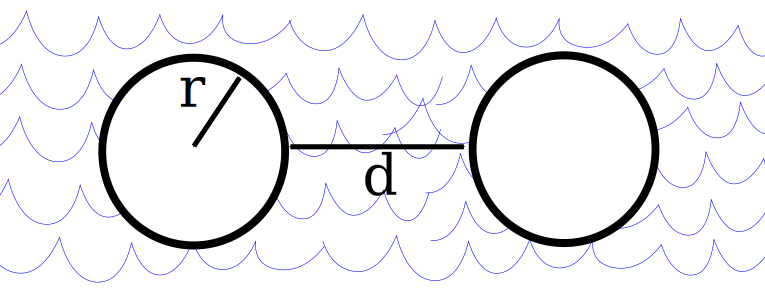
\includegraphics[width=\columnwidth]{figs/rods-diagram}
\end{center}
\caption{ Cross section schematic for two hydrophobic rods immersed in water.
The radius and separation are shown.}
\label{fig:rods}
\end{figure}

\begin{figure}
\begin{center}
\includegraphics[width=\columnwidth]{figs/density-rods-in-water}
\end{center}
\caption{ Density profiles illustrating the transition from vapor 
to liquid water between the rods. The radius is 0.5~nm, the top figure is 
at a separation of 0.5~nm and the
bottom is 0.6~nm. Figure~\ref{fig:rods-energy-vs-distance} shows
the energy for these and other separations.}
\label{fig:density-rods}
\end{figure}

To determine the critical separation, we start by considering a macroscopic surface
tension model where the free energy in the macroscopic limit is given by 
\begin{equation}
F = \gamma A + pV
\end{equation}
The first term describes the surface energy and the second term
is the work needed to create a cavity of volume $V$. Since this pressure term
scales with volume, it can be neglected relative to the surface term provided
the length scale is small compared with $\frac{\gamma} p$. At room temperature,
the value of $\frac{\gamma} p$ is equal to about $20~\mu m$ which is
much larger than any of the solutes we study. We expect that for those
larger radius 
rods, the water on the sides of the 'stadium' configuration will bow inward 
between the rods and the density will reduce to vapor near the center
point where the rods are closest to each other.

Starting from the surface energy term, we can calculate the 
free energy per length, which is equal to the circumference multiplied 
by the surface tension. The force per length is the derivative of this
with respect to the separation. 
We approximate the circumference of the stadium-shape by
\begin{equation}
C_{s} = 2\pi r +4r+2d
\end{equation}
and so the force per length is equal to $2\gamma$.

This is consistent with the calculation of the surface tension in
Figure~\ref{fig:surface-tension} (72~mN/m) and the force per length
found from the slopes of the curves in Figure
~\ref{fig:rods-energy-vs-distance} (144~mN/m)  which
compares the free energy per length for rods of several different
radii. This agreement indicates that even though the rods are nanoscale, the
water molecules will ``see'' them classically.  For large $d$, the rods 
simply act like two separate single rods in water and the energy will
reach an asymptote determined by the effective surface tension (shown in 
Figure~\ref{fig:energy-vs-diameter}). In Figure
~\ref{fig:rods-energy-vs-distance}, we see that for small $d$ all the rods 
have the same behavior with a positive linear relationship
between free energy per length and separation during the initial state 
with vapor between them. This indicates that the force 
per length on the rods is constant, and surprisingly independent of separation.

To estimate how the transition from vapor to liquid between the rods depends on their 
radius, we will again use the aforementioned model and propose that 
the critical separation, $d_c$, will occur when the free energies are equal. This 
corresponds to equating the circumference of the stadium-shape (see 
top of Figure~\ref{fig:density-rods}) and the circumference of the two rods (see bottom
of Figure~\ref{fig:density-rods}), which results in
\begin{equation}
d_c = (\pi-2)r.\label{criticalseparation}
\end{equation}
The predicted and actual computed values for $d_c$ are shown graphically in 
Figure~\ref{fig:rods-energy-vs-distance} where there is a transition
between the sloped and flat portion of each plot. They match fairly well for the 
0.5~-~1.0~nm rods with differences between 1.3~-~5.5\% and we hypothesize that larger radii rods
would also follow this trend, but smaller rods are likely to have a different
relationship with the surrounding water molecules. This may explain why the critical
separation result for a radius of 0.3~nm does not match the prediction
well (32\% difference).

\begin{figure}
\begin{center}
\includegraphics[width=\columnwidth]{figs/rods-energy-vs-distance}
\end{center}
\caption{ Free energy of hydration (also known as the potential of mean force) 
versus separation for two hydrophobic rods ranging in radius from
0.3~nm to 1.0~nm.
All were arbitrarily offset to zero at large separations for ease of comparison. The
transition corresponds to the phase change from
vapor to liquid between the rods as pictured in the density profiles in 
Figure~\ref{fig:density-rods}. }
\label{fig:rods-energy-vs-distance}
\end{figure}

Walther \emph{et al.}\cite{walther2004hydrodynamic} studied the interactions between two
carbon nanotubes, which are geometrically similar to our hydrophobic rods. 
They use molecular dynamics with Lennard-Jones potentials for
nanotubes of diameter 1.25~nm and separations ranging from about 0.3~nm to 1.5~nm.
They also find that a drying transition occurs, and find it to be at separations near
0.9~-~1.0~nm\cite{walther2004hydrodynamic}. This is larger than
what we find for hydrophobic rods of a similar size, as expected due to the carbon-carbon
and carbon-water interactions.

\subsection{Hydrophobic interactions of four rods}

\begin{figure}
\begin{center}
\includegraphics[width=\columnwidth]{figs/four-rods-energy-vs-distance}
\end{center}
\caption{ Free energy of hydration 
versus separation for four hydrophobic rods ranging in radius from
0.3~nm to 1.0~nm.
All were arbitrarily offset to zero at large separations. The
transition corresponds to the phase change from
vapor to liquid between the rods as pictured in the density profiles in 
Figure~\ref{fig:density-four-rods}. }
\label{fig:four-rods-energy-vs-distance}
\end{figure}

\begin{figure}
\begin{center}
\includegraphics[width=\columnwidth]{figs/density-four-rods}
\end{center}
\caption{ Density profiles illustrating the transition from vapor 
to liquid water between four rods. The radius is 0.5~nm, the top figure is 
at a separation of 1.1~nm and the
bottom is 1.2~nm. Figure~\ref{fig:four-rods-energy-vs-distance} shows
the energy for these and other separations.}

\label{fig:density-four-rods}
\end{figure}

We simulate four hydrophobic rods in water using the same radii as our
two rods ($r = 0.3$~nm~-~$1.0$~nm) and
separation distances between $d = 0$~nm to $d = 3$~nm for nearest neighbor rods. We placed
the rods in a 'square' arrangement and observed a similar behavior as the two rods
where vapor is present in the space between the rods until a critical separation
where it becomes filled with water and the rods behave as separate single rods
(shown in Fig. \ref{fig:density-four-rods}).  Free energy per length
is plotted against rod separation in Figure
\ref{fig:four-rods-energy-vs-distance} with a slight disagreement of
the predicted force per unit length.

The 'rounded square' formed by the area of the four rods and the space
between them has a circumference estimated by
\begin{equation}
C_{rs} = 2 \pi r + 8r + 4d.
\end{equation}
As with the two rods, we equate this circumference with the total circumference of
the four separate rods. This gives a critical separation of
\begin{equation}
d_{c4} = \frac{3 \pi - 4}{2} r. \label{criticalfourrods}
\end{equation}
We see in Figure \ref{fig:four-rods-energy-vs-distance} that the $r = 0.3$~nm
rod has the largest difference between simulation and prediction with
a 23\% difference, and better agreement for larger radii rods (between 0.5\% and 5.6\%).

\subsection{Hydration energy of hard-sphere solutes}

\begin{figure}
\begin{center}
\includegraphics[width=\columnwidth]{figs/sphere-energy-vs-diameter}
\end{center}
\caption{ Free energy versus radius for a single hydrophobic sphere
  immersed in water. This should have an asymptote equal to the
  surface tension at room temperature, and it agrees well with the
  surface tension in Figure~\ref{fig:surface-tension}. Results from a
  simulation of SPC/E water~\cite{huang2001shs} are shown as circles.
  The horizontal lines show the experimental and SPC/E bulk surface
  tension for water at standard atmospheric temperature and
  pressure. }
\label{fig:sphere-energy-vs-diameter}
\end{figure}

A common model of hydrophobic solutes is the \emph{hard sphere solute}
\cite{sedlmeier2011entropy}.  The effect of this solute is merely to create
a cavity within which the water may not penetrate.  This is the
simplest possible solute, and will serve as a test case, which if
passed could lead to the ability to insert different chemicals into
aqueous solution, instead of a vapor cavity, in order to observe
biologically and chemically important aqueous solvation interactions.

As in the single rod, we begin by examining the free energy of
hydration, expressed in Figure~\ref{fig:sphere-energy-vs-diameter} as
the ratio of the energy of the cavity system to the surface area of
the cavity.  This \emph{effective surface tension}, approaches the
bulk surface tension as the cavity radius increases.  As with the
single rod, we see the analytically correct behavior in the limit of
small solutes.  We also plot the surface tension calculated using a
molecular dynamics simulation of SPC/E water\cite{huang2001shs}.  The
agreement is quite excellent, apart from the issue that the SPC/E
model for water significantly underestimates the surface tension of
water at room temperature\cite{vega2007surface}.

Figure~\ref{fig:density-sphere} shows the density profile for several
hard sphere radii, plotted together with the results of the same
SPC/E molecular dynamics simulation shown in
Figure~\ref{fig:sphere-energy-vs-diameter}\cite{huang2001shs}.  The
agreement with simulation is quite reasonable.  The largest
disagreement involves the density at contact, which according to the
contact value theorem cannot agree, since the free energies do not
agree.

\begin{figure}
\begin{center}
\includegraphics[width=\columnwidth]{figs/density-sphere}
\end{center}
\caption{ Density profiles around hard-sphere solutes of different radii. Predictions
  from our classical density-functional theory are in solid red, while
  the dotted line shows the result of a molecular dynamics simulation
  of SPC/E water~\cite{huang2001shs}.  }
\label{fig:density-sphere}
\end{figure}

\section{Conclusion}

The classical density functional we developed by combining fundamental-measure 
theory with SAFT is able to produce reasonable results for hydrophobic interactions.
We added the parameter $\lscale$ to the functional and fit it to the surface tension
at room temperature, which we find to be consistent with results for larger hydrophobic
rods. 

The free energy per area for water surrounding a hydrophobic rod shows the
expected behavior with an asymptote equal to the surface tension.
Based on this result, we expect to be
able to classically describe a single rod with a radius of about 0.5~nm or larger. 
For two hydrophobic rods surrounded by water, we see a transition from a vapor-filled
stadium shape to two rods with liquid between them. A
classical treatment of the critical separation for this transition
works well for pairs of rods with radii larger than 0.5~nm.  Further evidence for the
accuracy of this classical treatment is the calculation of the force on the
stadium shape. The force per length is constant and equal to twice the
surface tension. A similar system with four hydrophobic rods exhibited the same
behavior while simulations of hydrophobic spheres agrees with
SPC/E calculations.

For the hydrophobic systems studied, this functional is more computationally 
efficient than molecular dynamics. This allows for future work
involving hydrophilic interactions with more complex electrostatic interactions.


\bibliography{paper}% Produces the bibliography via BibTeX.

\end{document}
